\chapter{Optimising Towards Unlikelihood: Data-Divergent Fine-Tuning of Generative Neural Networks}
\label{ch:divergent}

This chapter details experiments in the divergent fine-tuning of pretrained models, away from the likelihood of modelling data towards generating novel, unseen data distributions. 
The work in this chapter was first published in the paper \textit{Amplifying The Uncanny} was published at the 8th Conference on Computation, Communication, Aesthetics \& X (xCoAx) \citep{broad2020amplifying}. 
These experiments was the first peer-reviewed and published attempt at doing this (to the best of my knowledge), other approaches to divergent fine-tuning are detailed in \S \ref{survey:divergent}. 
It should be noted that the results presented here are not the exact results first shared in \cite{broad2020amplifying}. The experiments were re-run, so that more data could be logged, and more variations of parameter settings and loss functions could be compared.

\section{Motivation}
\label{c4:sec:motivation}

Following the work presented in Chapter \ref{ch:unstable_eq}, I was motivated to explore further the possibility of training generative neural networks without data. 
However, given the rather idiosyncratic nature of the arrangements of neural networks and loss functions presented in the last chapter, I wanted to pursue an approach that was more deliberate, with experiments that could be repeated by others more easily. 

Instead of training neural networks completely from random initialisation, I wanted find to new ways to fine-tune pre-trained models using novel loss functions and auxillary networks. 
The reasoning for this was that, it was clear, based on experiments such as deepdream (CITE) and tom whites perception engines (CITE), that CNN-based computer vision models had powerful representations baked into them, that could be optimised towards with gradient based optimisation in generative contexts.
My intuition was that if pretrained image recognition models could be used for generating individual images, then they also be used for fine-tuning existing generative models, in a data-divergent fashion.

Given the prohibitive amount of computational resources needed to train the then state-of-the-art (SOTA) models such as BigGAN (CITE) and StyleGAN (CITE) from scratch at the time, and the increasingly common practice of fine-tuning and transfer learning being used by creative people who wanted to work with high fidelity models (CITE). 
Instead of training from scratch, using pre-trained models to be fine-tuned in divergent ways was something that I could experiment much more rapidly. 
It also allowed for the alteration of existing learned features in a generator, to converge to a set of learned parameters for totally novel and divergent data distributions, in ways that diverge directly from the original training data (\S \ref{c4:sec:second-exp}). 

% Like Chapter \ref{ch:unstable_eq}, this work in this chapter is an adaptation of the traditional GAN adversarial training. 

\section{Method}
\label{c4:sec:method}

These experiments are done using the pre-trained checkpoints of the original StyleGAN trained on the FFHQ dataset \citep{karras2019style}. 
Three different checkpoints were used: one at 256x256 resolution, one at 512x512 resolution, and one at 1024x1024 resolution. 
These different checkpoints at different resolutions were available as the original StyleGAN implemented the progressive growing training method first used in \cite{karras2017progressive}.
The checkpoints used were not the official StyleGAN models released by NVIDIA, but instead a PyTorch reimplementation by \cite{rosinality2019style}.
This alternative implementation was used because the publicly available checkpoints contained both the frozen weights of the generator and the discriminator.\footnote{The NVIDIA official releases of StyleGAN weights only have the checkpoints of the generator}.

The standard GAN training objective is:

\begin{equation} 
\min_{G}\max_{D}\mathbb{E}_{x\sim p_{\text{data}}(x)}[\log{D(x)}] +  \mathbb{E}_{z\sim p_{\text{z}}(z)}[1 - \log{D(G(z))}]
\end{equation}

Where the generator network $G$ is trying to minimise the likelihood of it's generated samples being classified as fake, whereas the discriminator is optimised to maximise classification accuracy between real data samples and fake (generated) sampels.
The modification in this training regime is to, invert this loss function and instead optimised the generator toward maximising the likelihood that it's generated samples are correctly classified as being fake:

\begin{equation} 
  \max_{G}\mathbb{E}_{x\sim p_{\text{data}}(x)}[\log{D(x)}] +  \mathbb{E}_{z\sim p_{\text{z}}(z)}[1 - \log{D(G(z))}]
  \label{eq:inverted-adv-loss}
  \end{equation}

In this procedure, there is no training objective for the discriminator. 
The weights of the discriminator are kept frozen, and the network is simply used to calculated the loss function for the generator.
Figure \ref{fig:c4:gan-diagrams} shows visually the difference betwen the standard GAN training regime, and this modified fine-tuning procedure. 

\begin{figure}[!htbp]
  \centering
  \subfloat[]{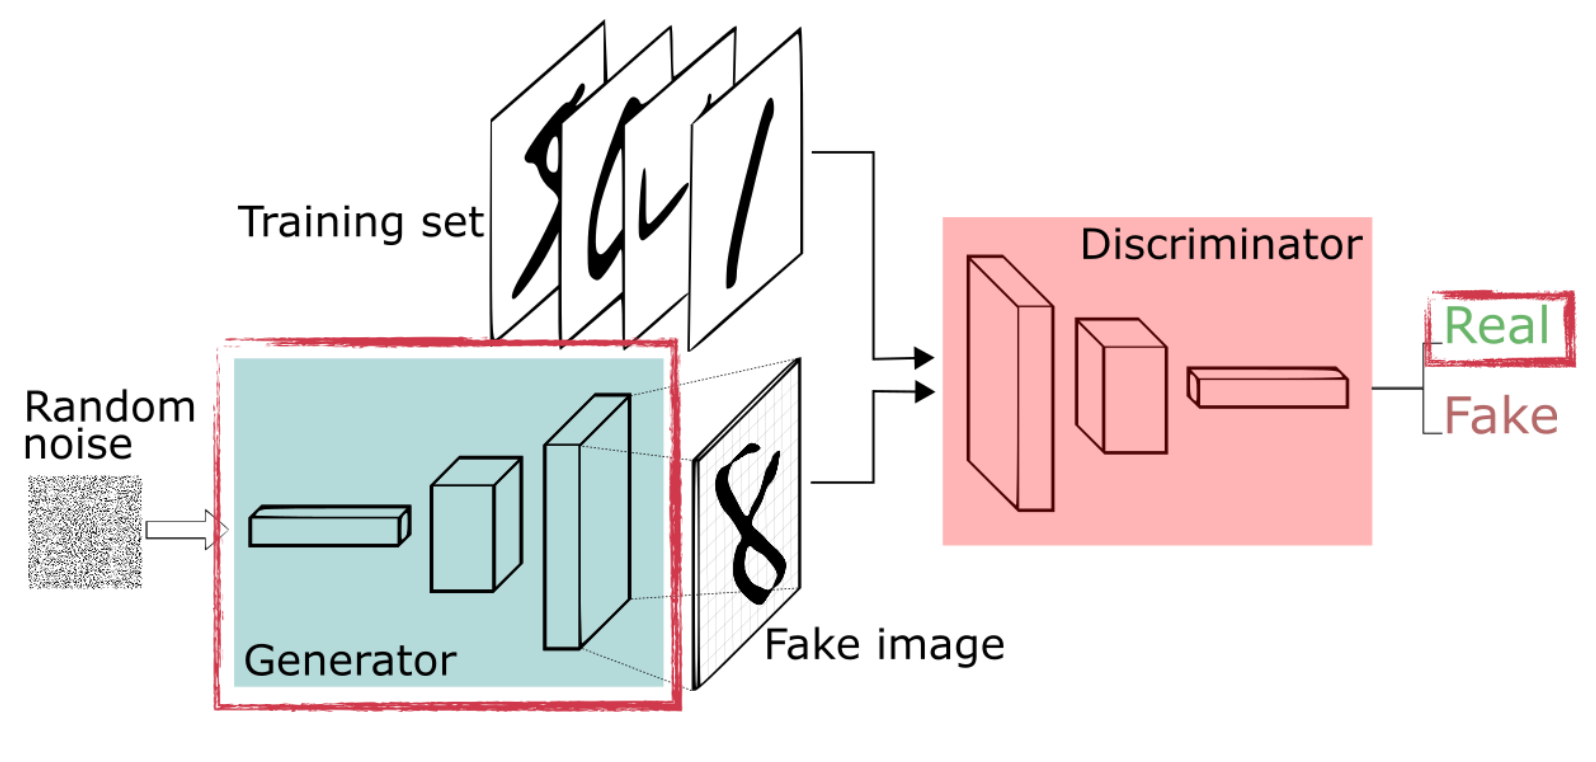
\includegraphics[width=1\textwidth]{figures/c4_divergent/diagrams/normal-gan-training.png}}
  \hfill
  \subfloat[]{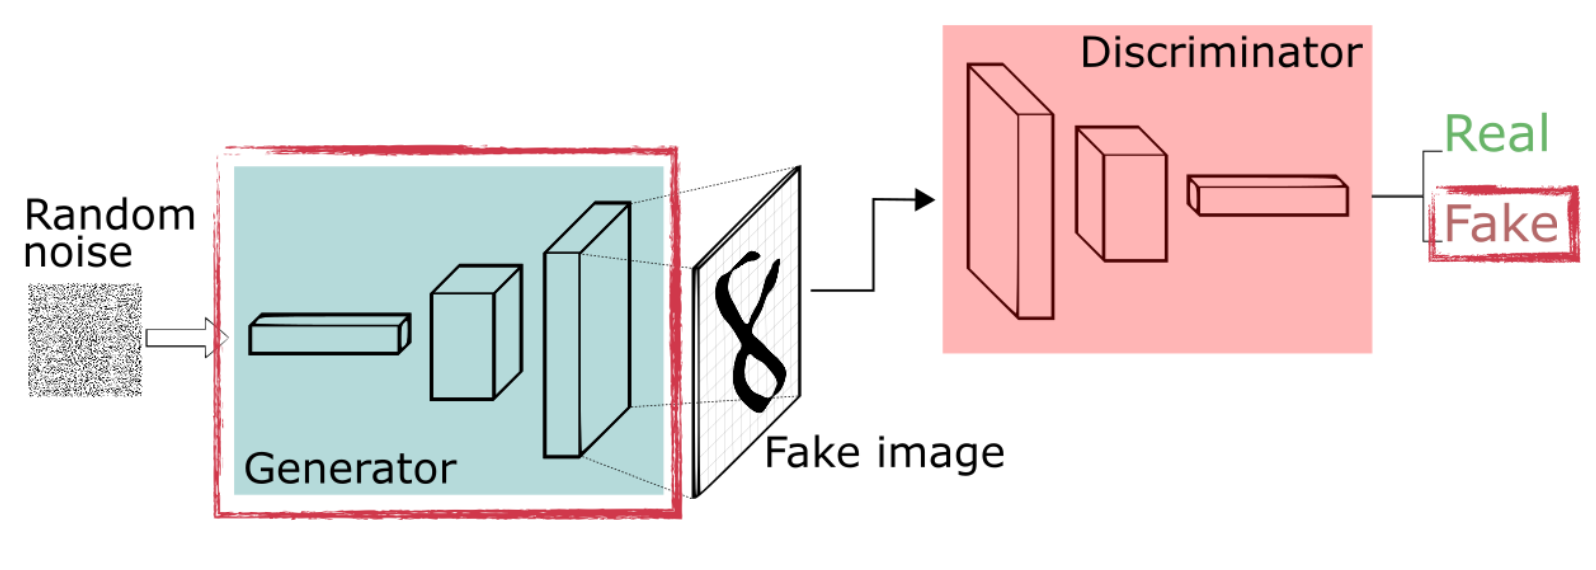
\includegraphics[width=1\textwidth]{figures/c4_divergent/diagrams/inverted-gan-loss.png}}
  \caption[Adversarial and inverted adversarial loss diagram]{Diagrams showing the standard GAN training regime with the loss that the generator is optimised towards (a), and the inverted adversarial loss fine-tuning procedure with the alternative loss for the generator network (b).}
  \label{fig:c4:gan-diagrams}
\end{figure}

In a second set of expiriments this loss is modified to take the natural logarithm of the modified GAN loss:

\begin{equation} 
  \max_{G}\log(\mathbb{E}_{x\sim p_{\text{data}}(x)}[\log{D(x)}] +  \mathbb{E}_{z\sim p_{\text{z}}(z)}[1 - \log{D(G(z))}])
  \label{eq:ln-inverted-adv-loss}
  \end{equation}

The results from this operation can be seen in \S \ref{c4:sec:log-loss}.

For each model checkpoint (256,512,1024) and for each loss function (inverse adversarial, log-inverse adversarial) three fine-tuning runs were performed with different parameters used for the batch size during training: 2, 4 \& 8.
Experimenting with different conditions for batch size was done in order to determine if this would have an impact on the generated results, as it is widely assumed that increasing the batch size improves visual fidelity in the standard GAN training regime. 

\section{Results}
\label{c4:sec:results}

This section shows the results of the fine-tuning training procedure. 
It is divded into two sub-sections the first (\S \ref{c4:sec:og-loss}) shows the results of the standard inverted adversarial loss (Equation \ref{eq:inverted-adv-loss}), the second (\S \ref{c4:sec:log-loss}) shows the results for the natural logarithm of the inverted adversarial loss (Equation \ref{eq:ln-inverted-adv-loss}).

\subsection{Inverted Adversarial Loss}
\FloatBarrier

This section shows the results of the standard inverted adversarial loss (Equation \ref{eq:inverted-adv-loss}). For all of these experiments with this loss function the fine-tuning procedure was performed for 1000 iterations.
Figures \ref{fig:c4:256-OG-samples} \& \ref{fig:c4:256-OG-losses} show the generated samples and losses during fine tuning for the 256x256 checkpoint.
Figures \ref{fig:c4:512-OG-samples} \& \ref{fig:c4:512-OG-losses} show the generated samples and losses during fine tuning for the 512x512 checkpoint.
Figures \ref{fig:c4:1024-OG-samples} \& \ref{fig:c4:1024-OG-losses} show the generated samples and losses during fine tuning for the 1024x1024 checkpoint.

\label{c4:sec:og-loss}
\begin{figure}[!htbp]
    \centering
    \subfloat[]{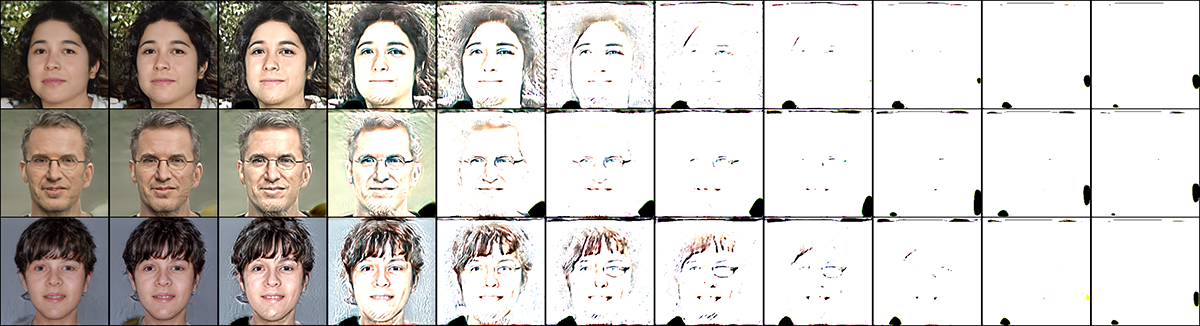
\includegraphics[width=1\textwidth]{figures/c4_divergent/gen-plots/OG/256/256-OG-2-Images-1000.png}}
    \hfill
    \subfloat[]{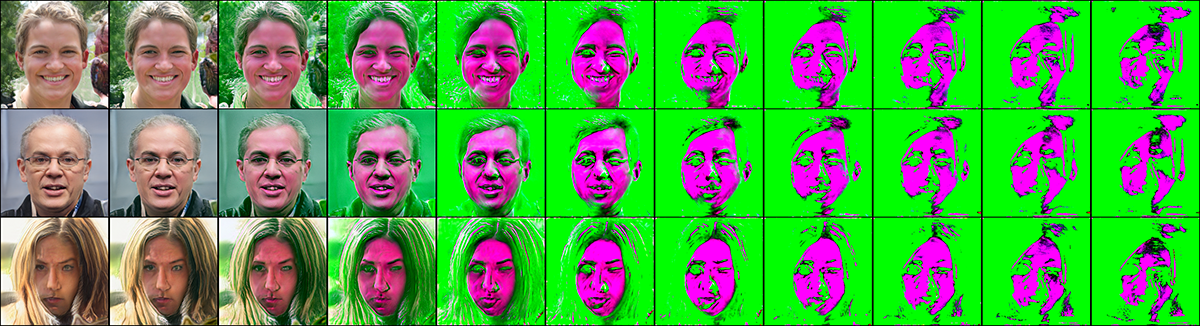
\includegraphics[width=1\textwidth]{figures/c4_divergent/gen-plots/OG/256/256-OG-4-Images-1000.png}}
    \hfill
    \subfloat[]{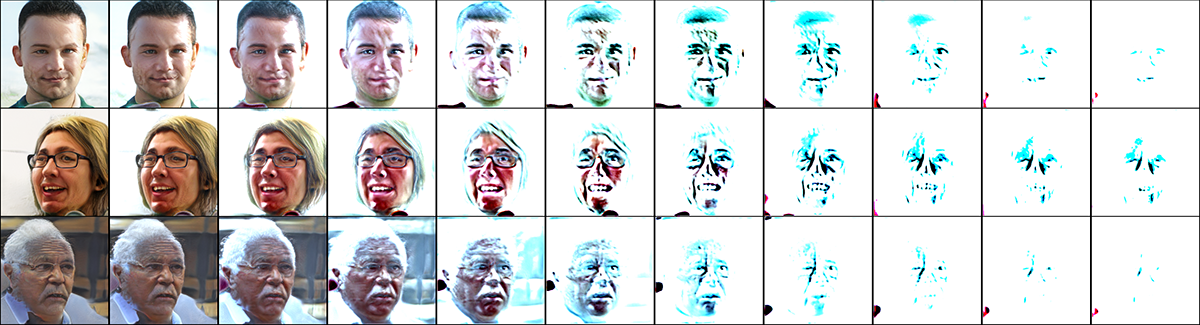
\includegraphics[width=1\textwidth]{figures/c4_divergent/gen-plots/OG/256/256-OG-8-Images-1000.png}}
    \caption[Samples of generations during fine-tuning procedure for 256x256 StyleGAN model with the inverted adversarial loss function]{Samples of generations during fine-tuning procedure for 256x256 StyleGAN model with the inverted adversarial loss function, at increments of 100, between training step 0-10000. (a) Results with batch size 2. (b) Results with batch size 4. (c) Results with batch size 8.}
    \label{fig:c4:256-OG-samples}
  \end{figure}

  \begin{figure}[!htbp]
    \centering
    \subfloat[]{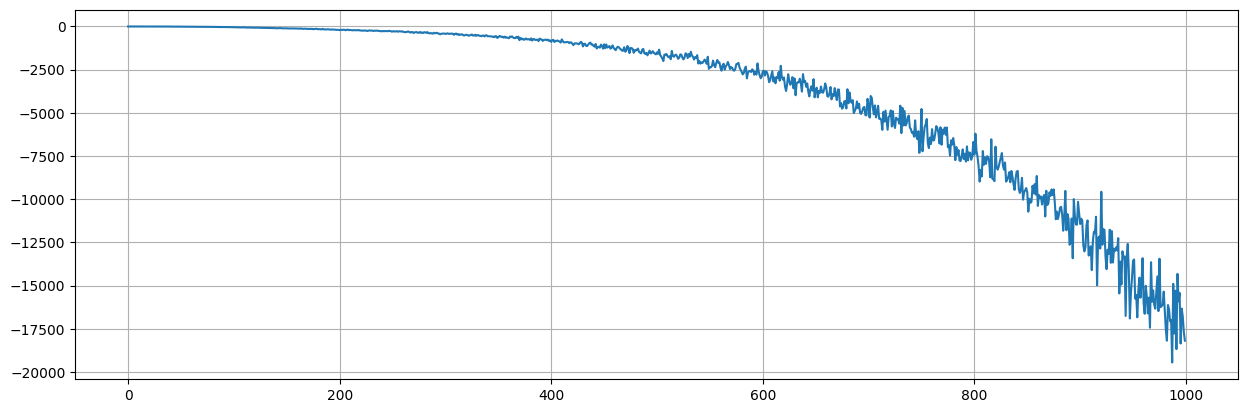
\includegraphics[width=0.8\textwidth]{figures/c4_divergent/loss-plots/OG/256/256-B2.png}}
    \hfill
    \subfloat[]{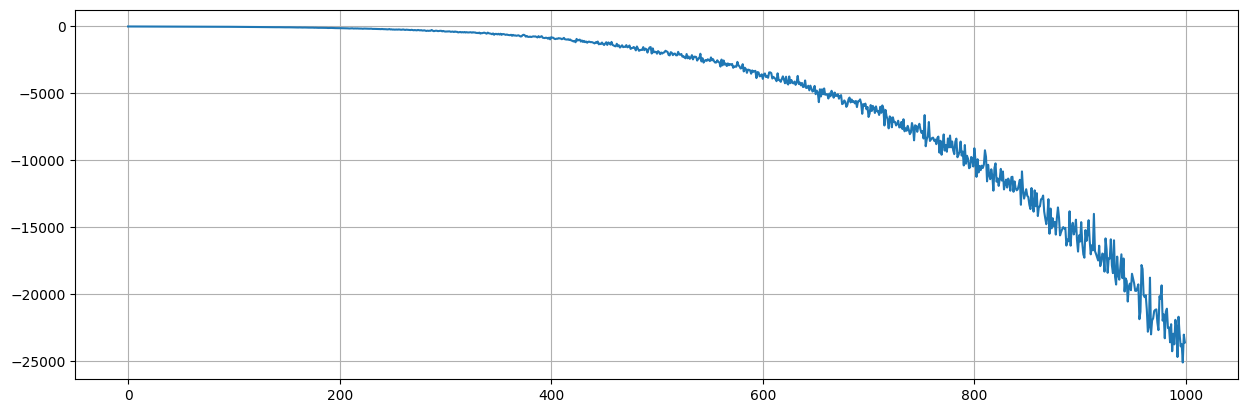
\includegraphics[width=0.8\textwidth]{figures/c4_divergent/loss-plots/OG/256/256-B4.png}}
    \hfill
    \subfloat[]{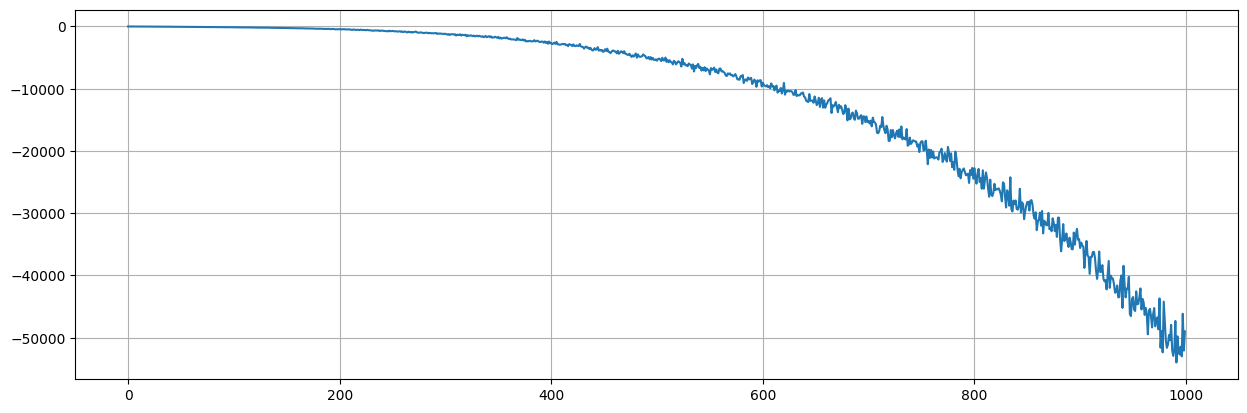
\includegraphics[width=0.8\textwidth]{figures/c4_divergent/loss-plots/OG/256/256-B8.png}}
    \caption[Loss plots for fine-tuning procedure for 256x256 StyleGAN model with the inverted adversarial loss function]{Loss plots for fine-tuning procedure for 256x256 StyleGAN model with the inverted adversarial loss function. (a) Results with batch size 2. (b) Results with batch size 4. (c) Results with batch size 8.}
    \label{fig:c4:256-OG-losses}
  \end{figure}

  \begin{figure}[!htbp]
    \centering
    \subfloat[]{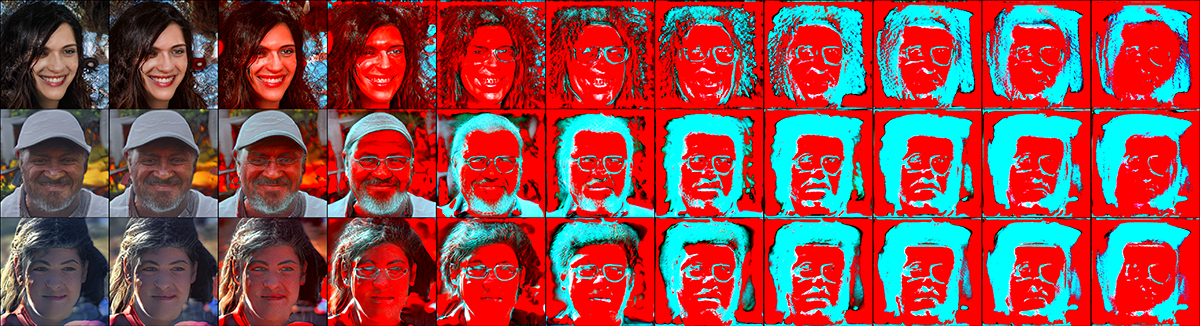
\includegraphics[width=1\textwidth]{figures/c4_divergent/gen-plots/OG/512/512-OG-2-Images-1000.png}}
    \hfill
    \subfloat[]{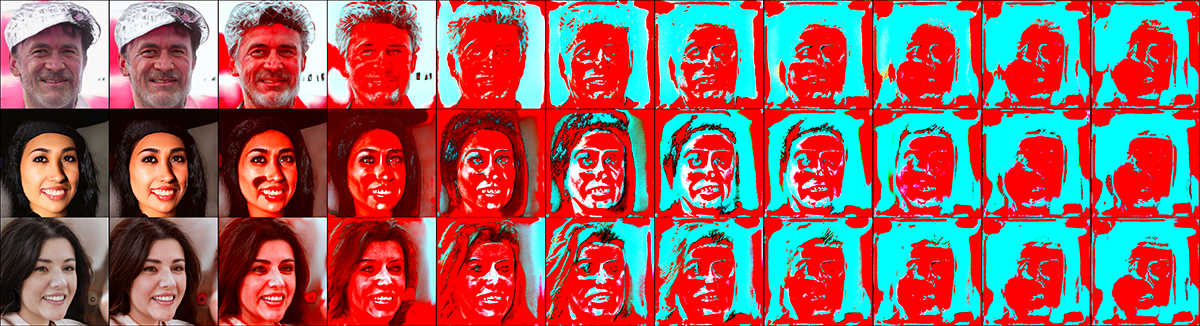
\includegraphics[width=1\textwidth]{figures/c4_divergent/gen-plots/OG/512/512-OG-4-Images-1000.png}}
    \hfill
    \subfloat[]{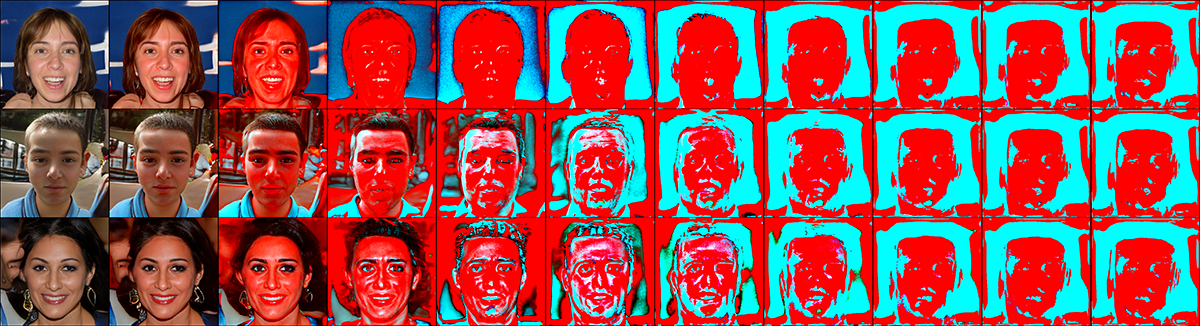
\includegraphics[width=1\textwidth]{figures/c4_divergent/gen-plots/OG/512/512-OG-8-Images-1000.png}}
    \caption[Samples of generations during fine-tuning procedure for 512x512 StyleGAN model with the inverted adversarial loss function]{Samples of generations during fine-tuning procedure for 512x512 StyleGAN model with the inverted adversarial loss function, at increments of 100, between training step 0-1000. (a) Results with batch size 2. (b) Results with batch size 4. (c) Results with batch size 8.}
    \label{fig:c4:512-OG-samples}
  \end{figure}

  \begin{figure}[!htbp]
    \centering
    \subfloat[]{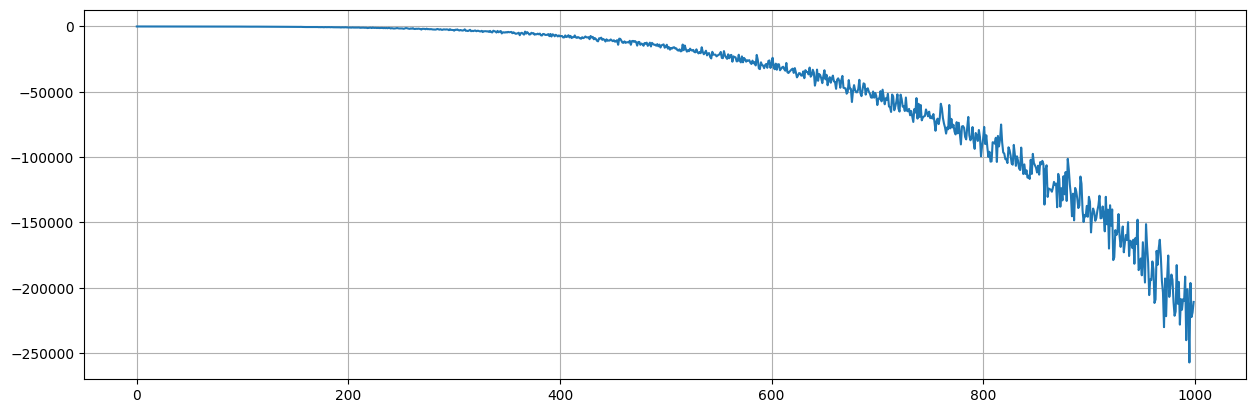
\includegraphics[width=0.8\textwidth]{figures/c4_divergent/loss-plots/OG/512/512-B2.png}}
    \hfill
    \subfloat[]{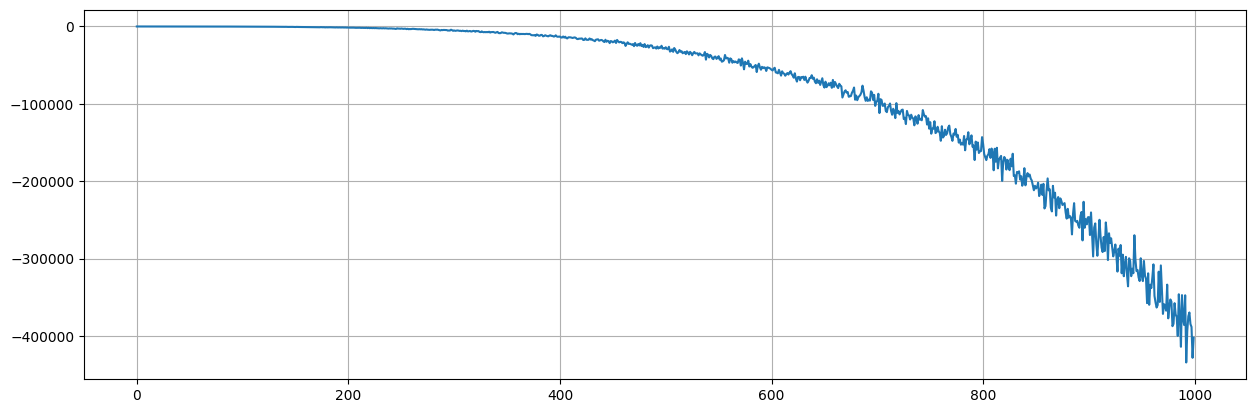
\includegraphics[width=0.8\textwidth]{figures/c4_divergent/loss-plots/OG/512/512-B4.png}}
    \hfill
    \subfloat[]{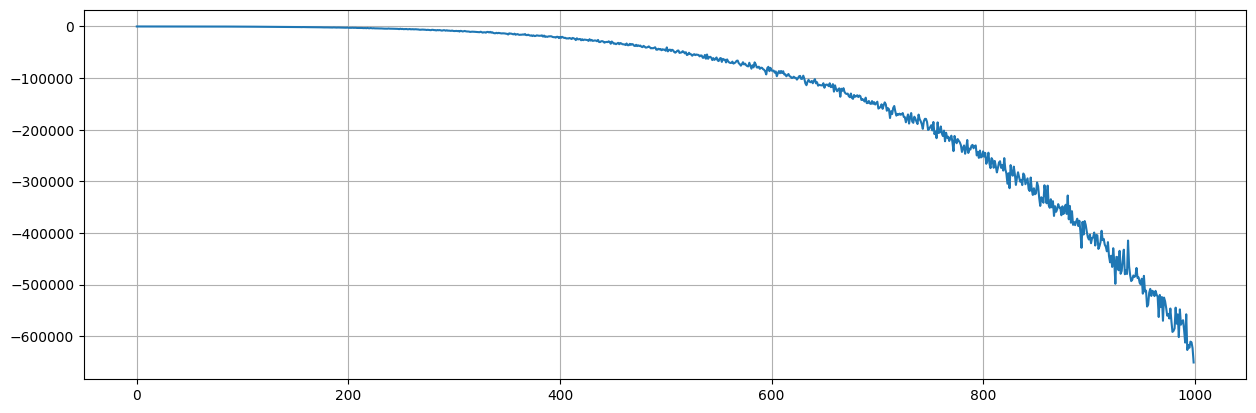
\includegraphics[width=0.8\textwidth]{figures/c4_divergent/loss-plots/OG/512/512-B8.png}}
    \caption[Loss plots for fine-tuning procedure for 512x512 StyleGAN model with the inverted adversarial loss function]{Loss plots for fine-tuning procedure for 512x512 StyleGAN model with the inverted adversarial loss function. (a) Results with batch size 2. (b) Results with batch size 4. (c) Results with batch size 8.}
    \label{fig:c4:512-OG-losses}
  \end{figure}

  \begin{figure}[!htbp]
    \centering
    \subfloat[]{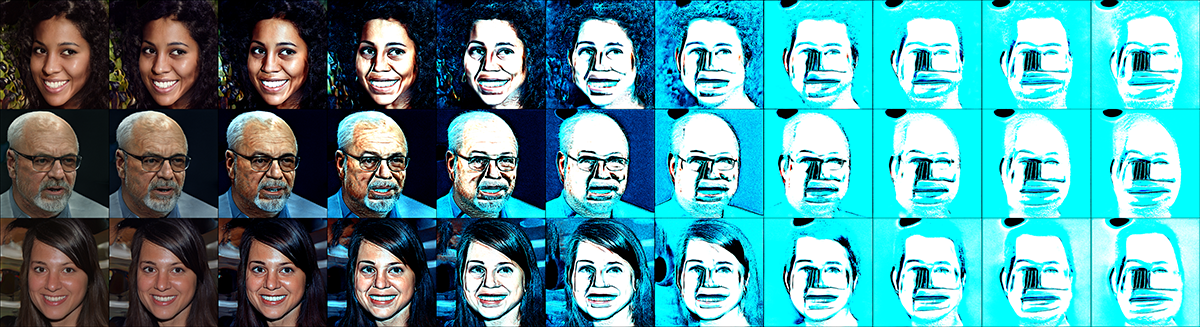
\includegraphics[width=1\textwidth]{figures/c4_divergent/gen-plots/OG/1024/1024-OG-2-Images-1000.png}}
    \hfill
    \subfloat[]{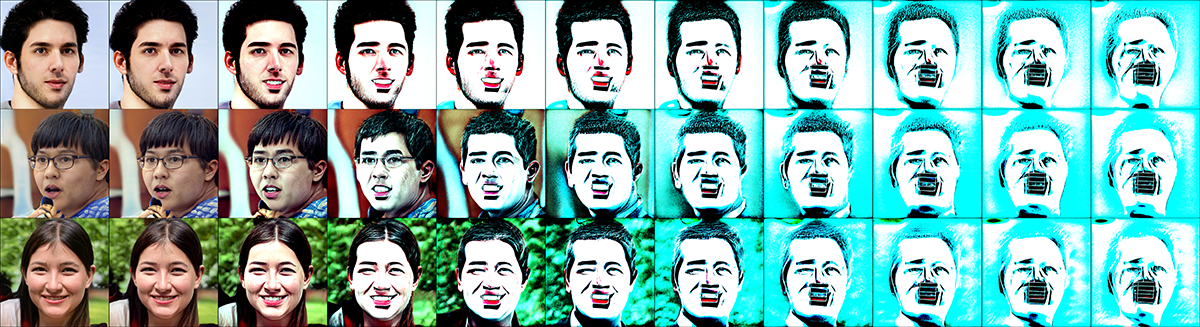
\includegraphics[width=1\textwidth]{figures/c4_divergent/gen-plots/OG/1024/1024-OG-4-Images-1000.png}}
    \hfill
    \subfloat[]{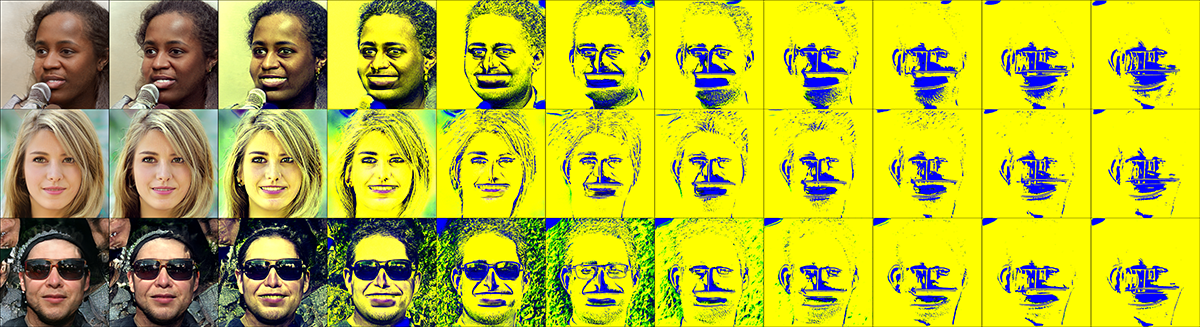
\includegraphics[width=1\textwidth]{figures/c4_divergent/gen-plots/OG/1024/1024-OG-8-Images-1000.png}}
    \caption[Samples of generations during fine-tuning procedure for 1024x1024 StyleGAN model with the inverted adversarial loss function]{Samples of generations during fine-tuning procedure for 1024x1024 StyleGAN model with the inverted adversarial loss function, at increments of 100, between training step 0-1000. (a) Results with batch size 2. (b) Results with batch size 4. (c) Results with batch size 8.}
    \label{fig:c4:1024-OG-samples}
  \end{figure}

  \begin{figure}[!htbp]
    \centering
    \subfloat[]{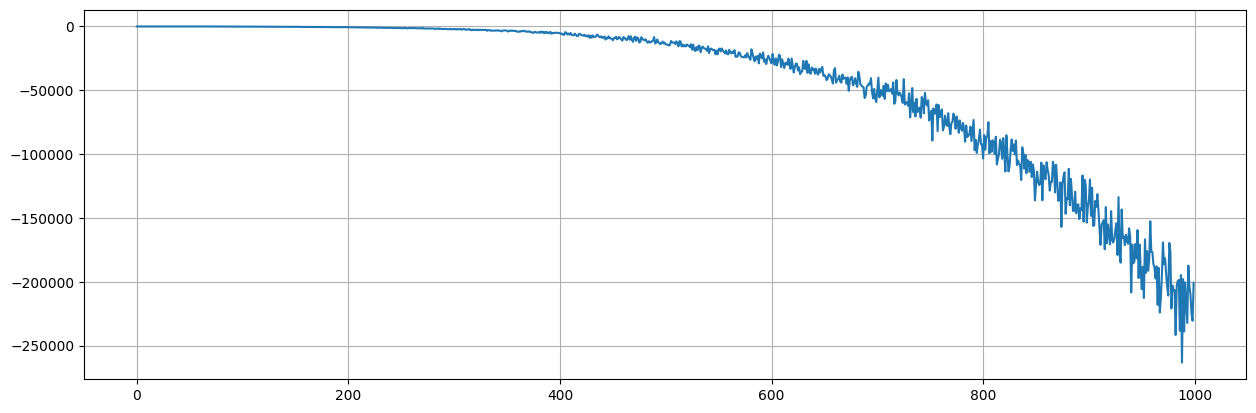
\includegraphics[width=0.8\textwidth]{figures/c4_divergent/loss-plots/OG/1024/1024-B2.png}}
    \hfill
    \subfloat[]{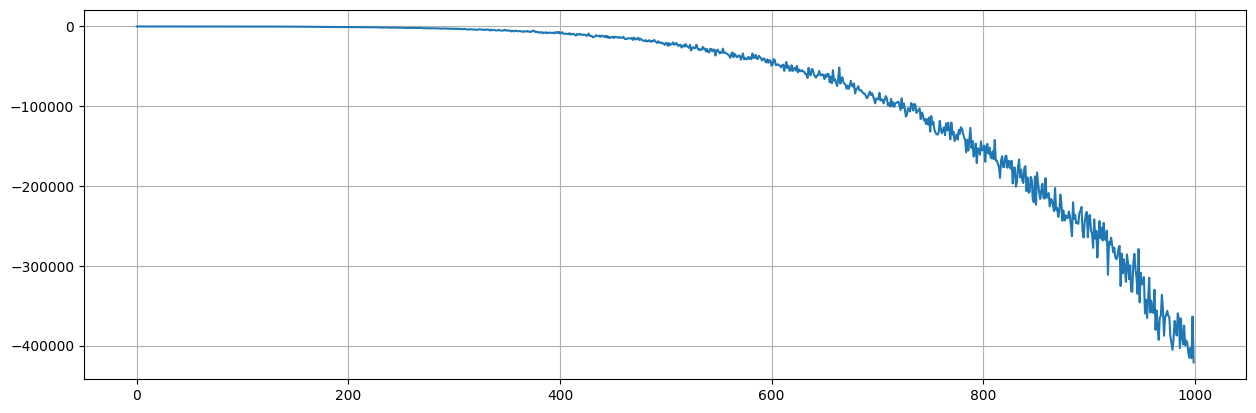
\includegraphics[width=0.8\textwidth]{figures/c4_divergent/loss-plots/OG/1024/1024-B4.png}}
    \hfill
    \subfloat[]{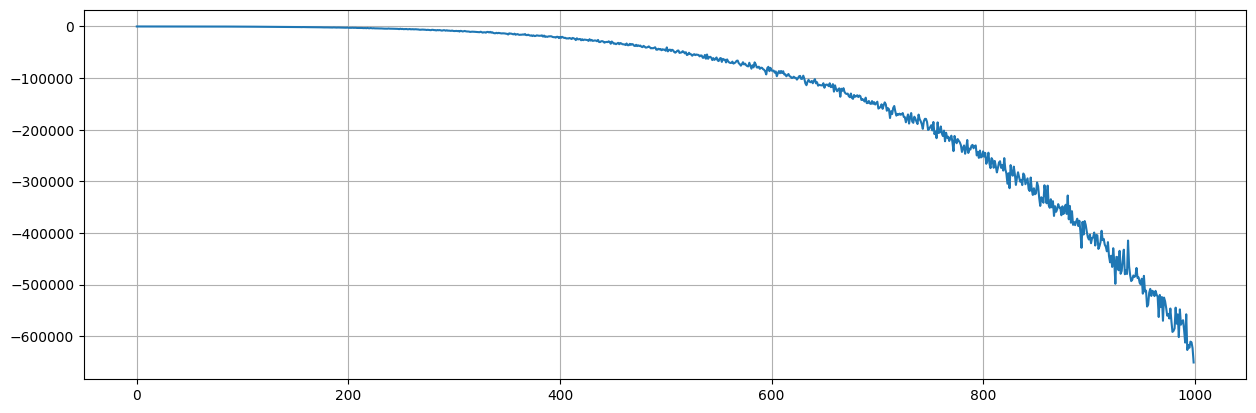
\includegraphics[width=0.8\textwidth]{figures/c4_divergent/loss-plots/OG/1024/1024-B8.png}}
    \caption[Loss plots for fine-tuning procedure for 1024x1024 StyleGAN model with the inverted adversarial loss function]{Loss plots for fine-tuning procedure for 1024x1024 StyleGAN model with the inverted adversarial loss function. (a) Results with batch size 2. (b) Results with batch size 4. (c) Results with batch size 8.}
    \label{fig:c4:1024-OG-losses}
  \end{figure}

\FloatBarrier

\subsection{Natural Logarithm of Inverted Adversarial Loss}
\label{c4:sec:log-loss}

This section shows the results of the standard inverted adversarial loss (Equation \ref{eq:ln-inverted-adv-loss}). For all of these experiments with this loss function the fine-tuning procedure was performed for 10000 iterations.
Figures \ref{fig:c4:256-LOG-samples} \& \ref{fig:c4:256-LOG-losses} show the generated samples and losses during fine tuning for the 256x256 checkpoint.
Figures \ref{fig:c4:512-LOG-samples} \& \ref{fig:c4:512-LOG-losses} show the generated samples and losses during fine tuning for the 512x512 checkpoint.
Figures \ref{fig:c4:1024-LOG-samples} \& \ref{fig:c4:1024-LOG-losses} show the generated samples and losses during fine tuning for the 1024x1024 checkpoint.

\begin{figure}[!htbp]
    \centering
    \subfloat[]{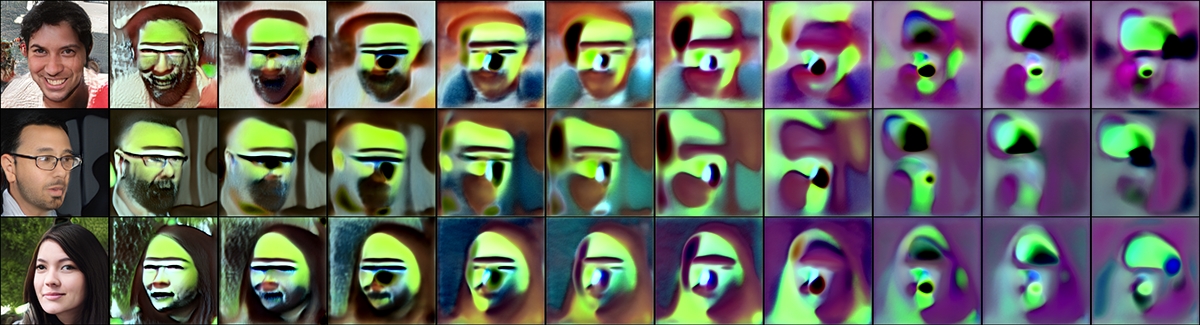
\includegraphics[width=1\textwidth]{figures/c4_divergent/gen-plots/LOG/256/256-LOG-2-Images-10000.png}}
    \hfill
    \subfloat[]{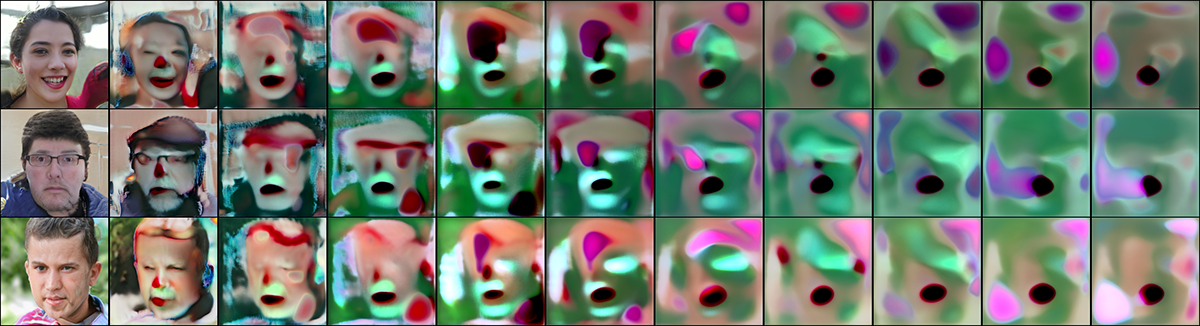
\includegraphics[width=1\textwidth]{figures/c4_divergent/gen-plots/LOG/256/256-LOG-4-Images-10000.png}}
    \hfill
    \subfloat[]{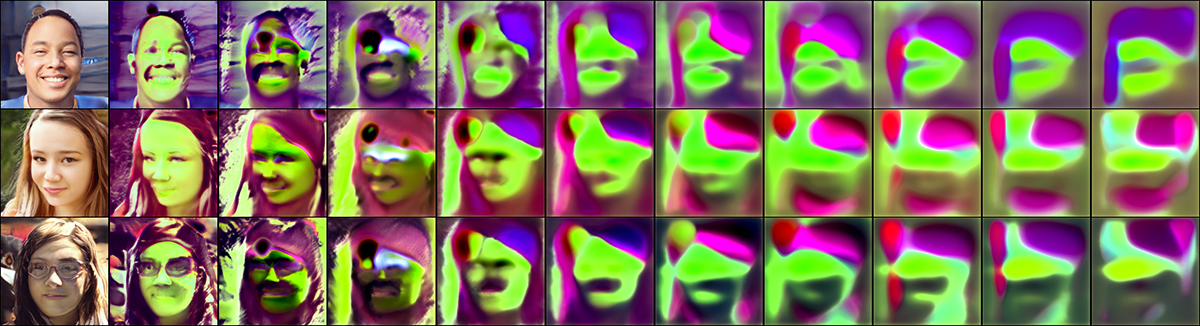
\includegraphics[width=1\textwidth]{figures/c4_divergent/gen-plots/LOG/256/256-LOG-8-Images-10000.png}}
    \caption[Samples of generations during fine-tuning procedure for 256x256 StyleGAN model with the natural logarithm of the inverted adversarial loss function]{Samples of generations during fine-tuning procedure for 256x256 StyleGAN model with the natural logarithm of the inverted adversarial loss function, at increments of 1000, between training step 0-10000. (a) Results with batch size 2. (b) Results with batch size 4. (c) Results with batch size 8.}
    \label{fig:c4:256-LOG-samples}
  \end{figure}

  \begin{figure}[!htbp]
    \centering
    \subfloat[]{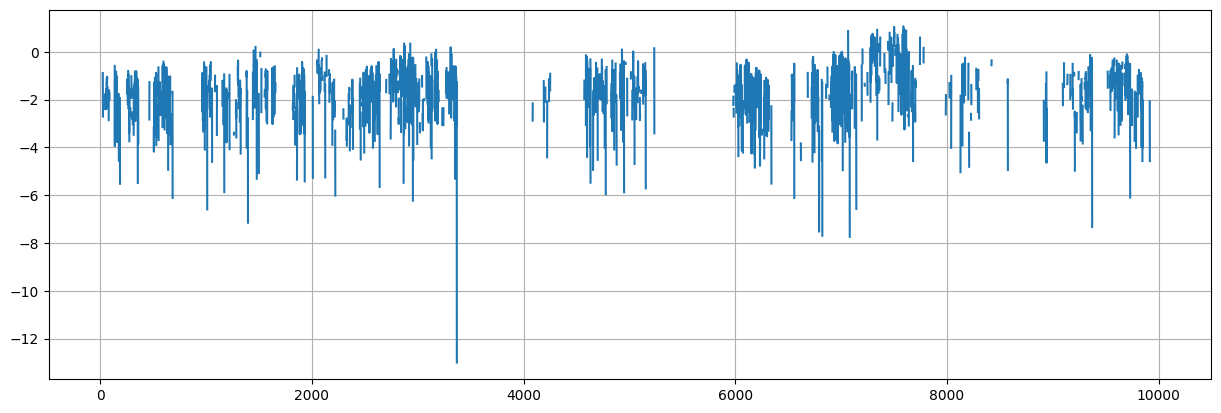
\includegraphics[width=0.8\textwidth]{figures/c4_divergent/loss-plots/LOG/256/256-B2.png}}
    \hfill
    \subfloat[]{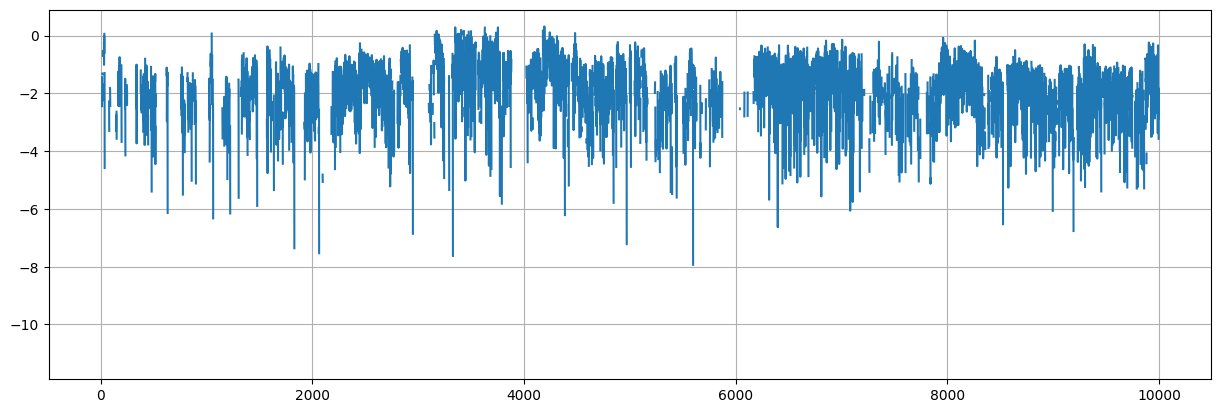
\includegraphics[width=0.8\textwidth]{figures/c4_divergent/loss-plots/LOG/256/256-B4.png}}
    \hfill
    \subfloat[]{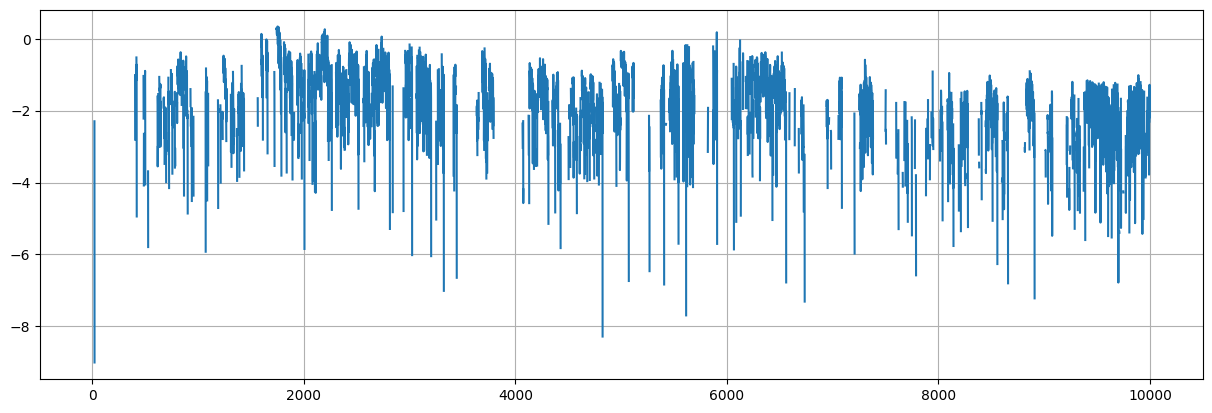
\includegraphics[width=0.8\textwidth]{figures/c4_divergent/loss-plots/LOG/256/256-B8.png}}
    \caption[Loss plots for fine-tuning procedure for 256x256 StyleGAN model with the natural logarithm of the inverted adversarial loss function]{Loss plots for fine-tuning procedure for 256x256 StyleGAN model with the natural logarithm of the inverted adversarial loss function. (a) Results with batch size 2. (b) Results with batch size 4. (c) Results with batch size 8. Note: gaps in the plot are where the loss was undefined from taking the log of a negative number.}
    \label{fig:c4:256-LOG-losses}
  \end{figure}

  \begin{figure}[!htbp]
    \centering
    \subfloat[]{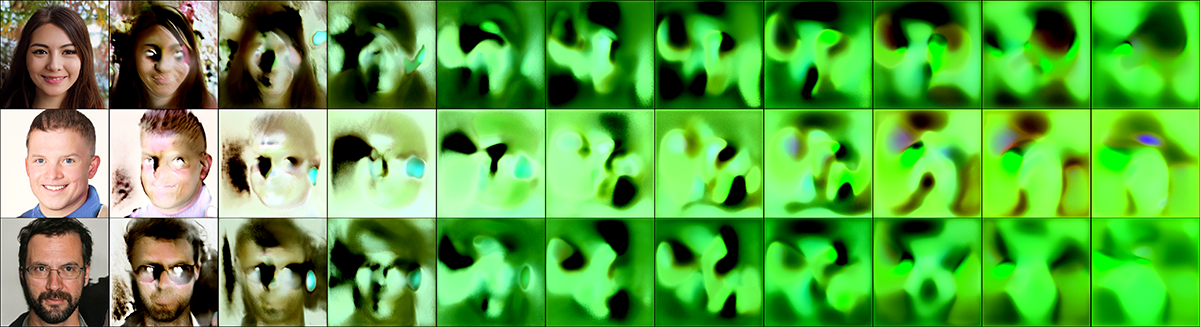
\includegraphics[width=1\textwidth]{figures/c4_divergent/gen-plots/LOG/512/512-LOG-2-Images-10000.png}}
    \hfill
    \subfloat[]{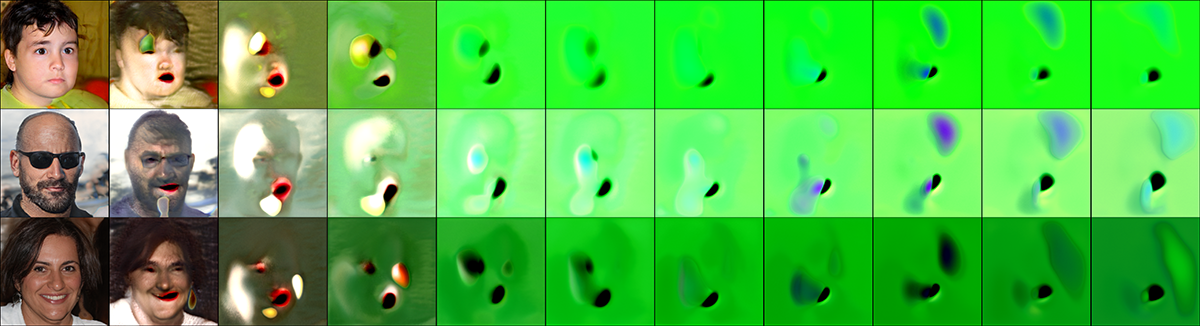
\includegraphics[width=1\textwidth]{figures/c4_divergent/gen-plots/LOG/512/512-LOG-4-Images-10000.png}}
    \hfill
    \subfloat[]{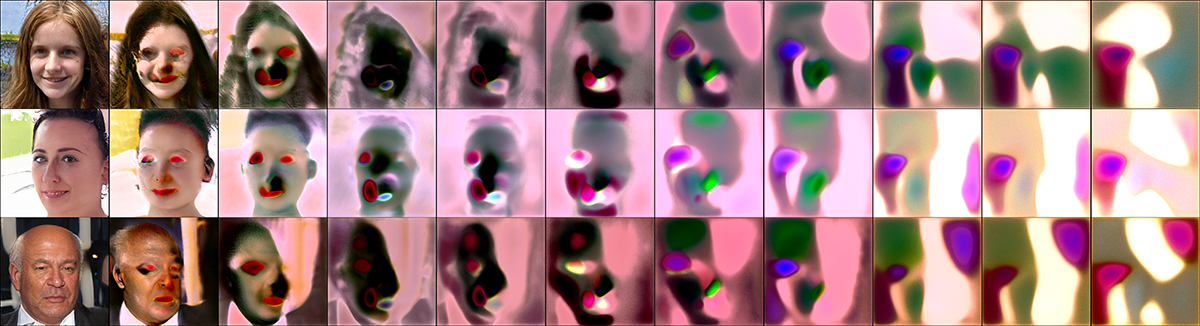
\includegraphics[width=1\textwidth]{figures/c4_divergent/gen-plots/LOG/512/512-LOG-8-Images-10000.png}}
    \caption[Samples of generations during fine-tuning procedure for 512x512 StyleGAN model with the natural logarithm of the inverted adversarial loss function]{Samples of generations during fine-tuning procedure for 512x512 StyleGAN model with the natural logarithm of the inverted adversarial loss function, at increments of 1000, between training step 0-10000. (a) Results with batch size 2. (b) Results with batch size 4. (c) Results with batch size 8.}
    \label{fig:c4:512-LOG-samples}
  \end{figure}

  \begin{figure}[!htbp]
    \centering
    \subfloat[]{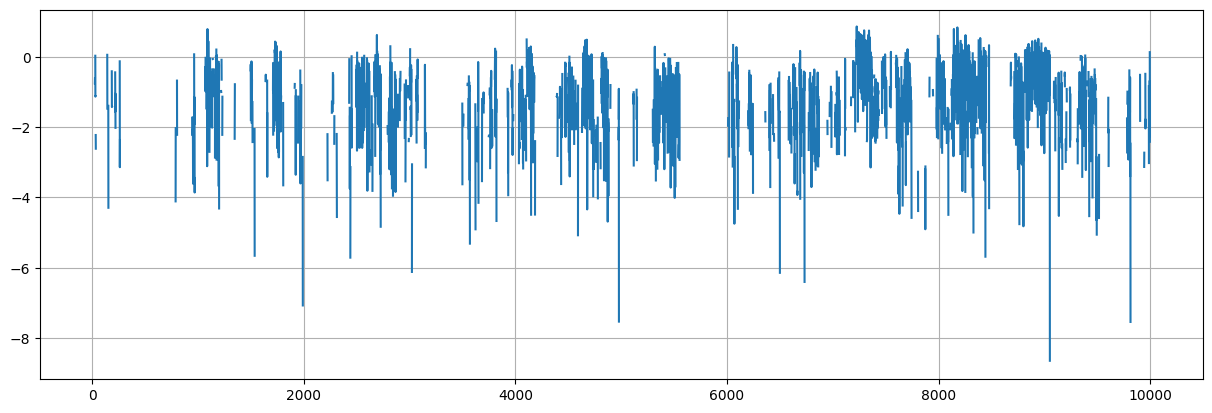
\includegraphics[width=0.8\textwidth]{figures/c4_divergent/loss-plots/LOG/512/512-B2.png}}
    \hfill
    \subfloat[]{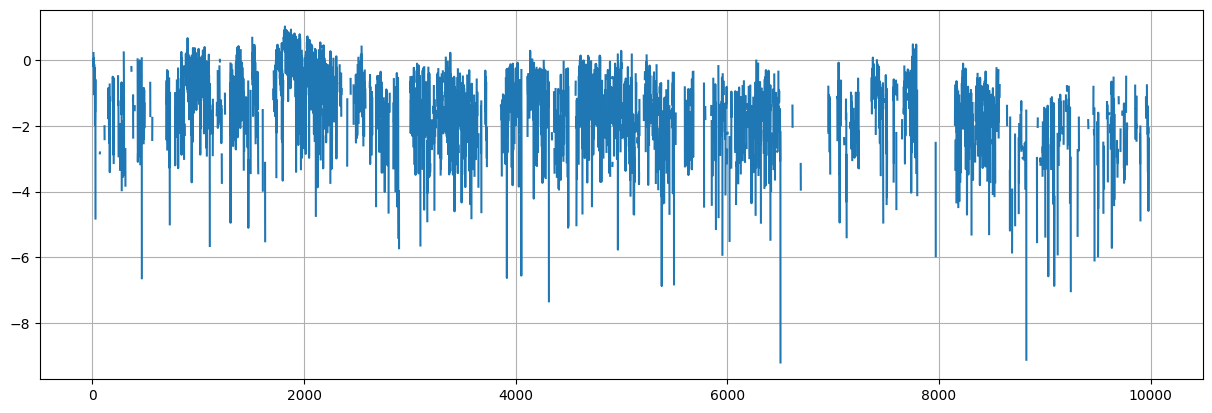
\includegraphics[width=0.8\textwidth]{figures/c4_divergent/loss-plots/LOG/512/512-B4.png}}
    \hfill
    \subfloat[]{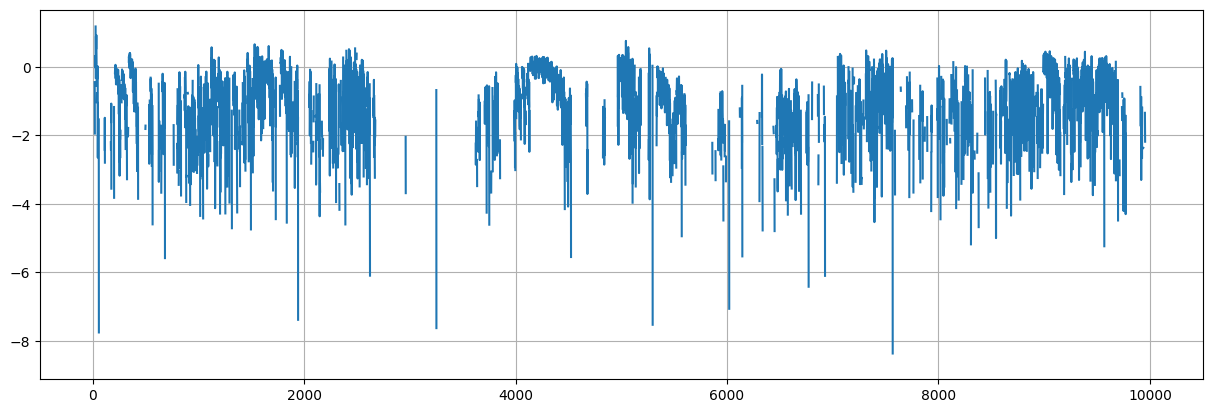
\includegraphics[width=0.8\textwidth]{figures/c4_divergent/loss-plots/LOG/512/512-B8.png}}
    \caption[Loss plots for fine-tuning procedure for 512x512 StyleGAN model with the natural logarithm of the inverted adversarial loss function]{Loss plots for fine-tuning procedure for 512x512 StyleGAN model with the natural logarithm of the inverted adversarial loss function. (a) Results with batch size 2. (b) Results with batch size 4. (c) Results with batch size 8. Note: gaps in the plot are where the loss was undefined from taking the log of a negative number.}
    \label{fig:c4:512-LOG-losses}
  \end{figure}

  \begin{figure}[!htbp]
    \centering
    \subfloat[]{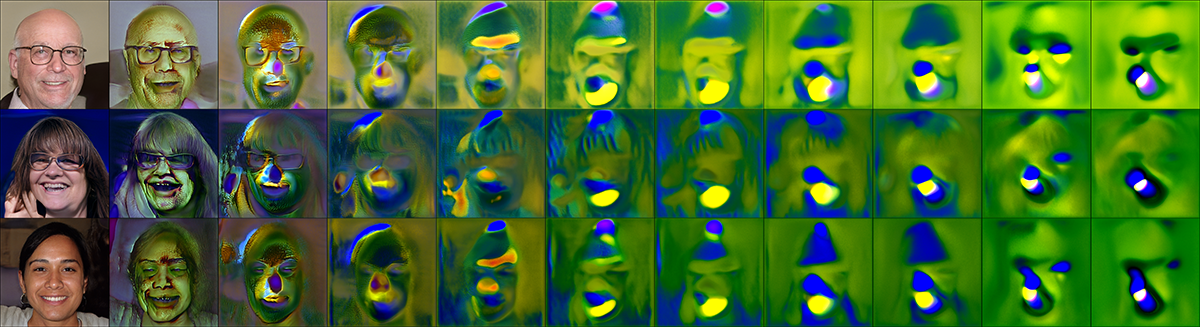
\includegraphics[width=1\textwidth]{figures/c4_divergent/gen-plots/LOG/1024/1024-LOG-2-Images-10000.png}}
    \hfill
    \subfloat[]{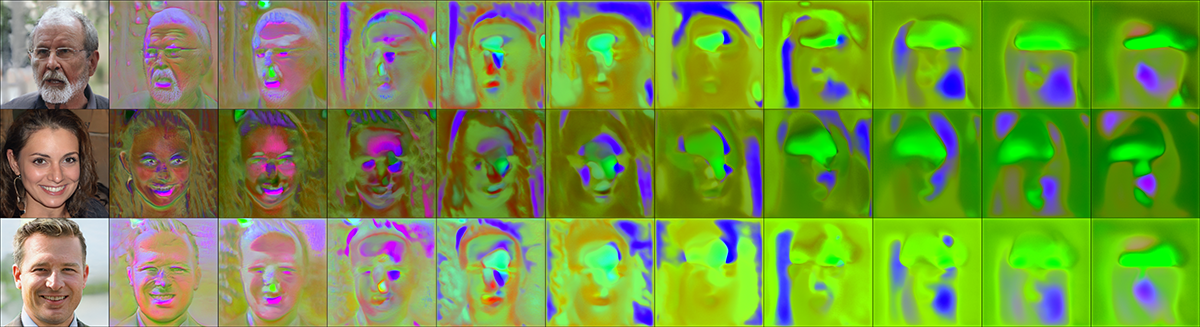
\includegraphics[width=1\textwidth]{figures/c4_divergent/gen-plots/LOG/1024/1024-LOG-4-Images-10000.png}}
    \hfill
    \subfloat[]{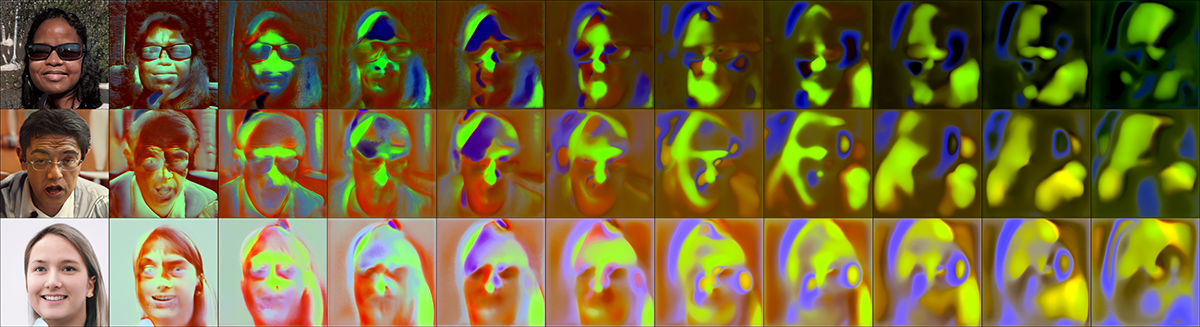
\includegraphics[width=1\textwidth]{figures/c4_divergent/gen-plots/LOG/1024/1024-LOG-8-Images-10000.png}}
    \caption[Samples of generations during fine-tuning procedure for 1024x1024 StyleGAN model with the natural logarithm of the inverted adversarial loss function]{Samples of generations during fine-tuning procedure for 1024x1024 StyleGAN model with the natural logarithm of the inverted adversarial loss function, at increments of 1000, between training step 0-10000. (a) Results with batch size 2. (b) Results with batch size 4. (c) Results with batch size 8.}
    \label{fig:c4:1024-LOG-samples}
  \end{figure}

  \begin{figure}[!htbp]
    \centering
    \subfloat[]{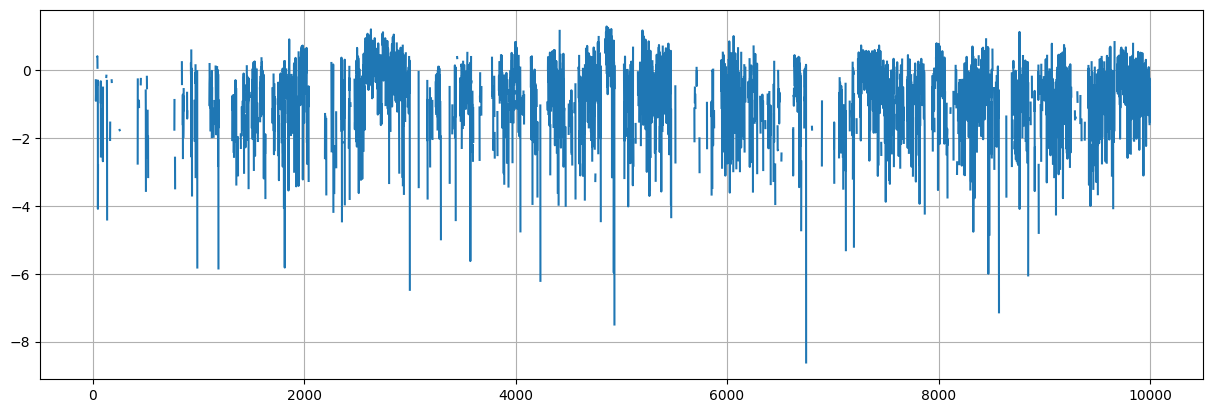
\includegraphics[width=0.8\textwidth]{figures/c4_divergent/loss-plots/LOG/1024/1024-B2.png}}
    \hfill
    \subfloat[]{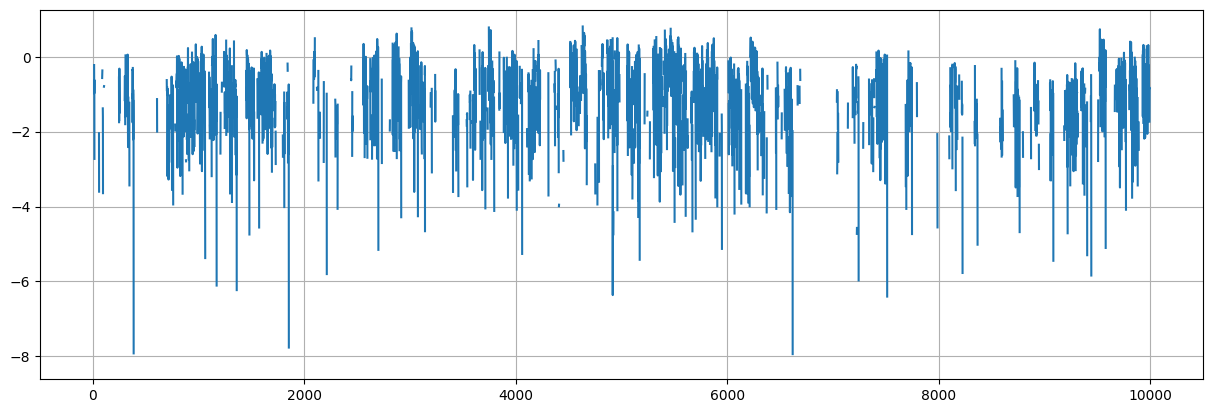
\includegraphics[width=0.8\textwidth]{figures/c4_divergent/loss-plots/LOG/1024/1024-B4.png}}
    \hfill
    \subfloat[]{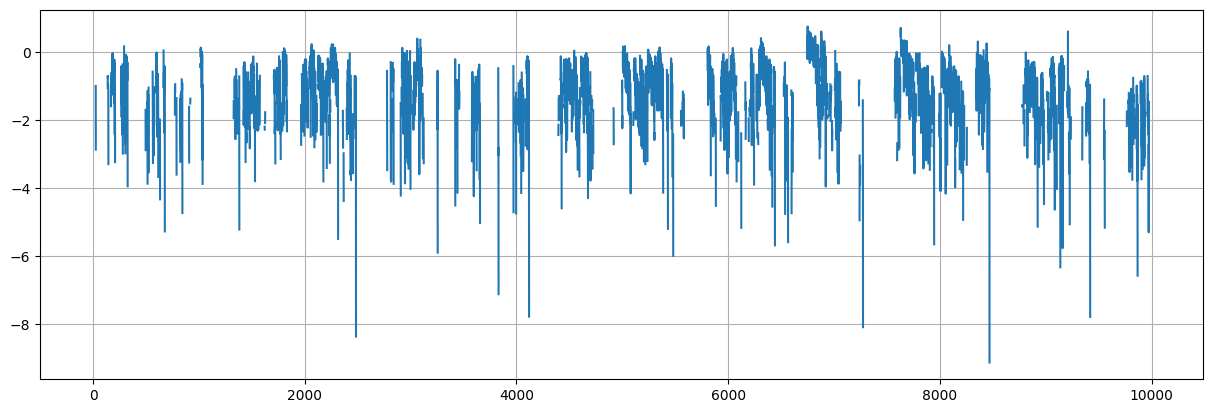
\includegraphics[width=0.8\textwidth]{figures/c4_divergent/loss-plots/LOG/1024/1024-B8.png}}
    \caption[Loss plots for fine-tuning procedure for 1024x1024 StyleGAN model with the natural logarithm of the inverted adversarial loss function]{Loss plots for fine-tuning procedure for 1024x1024 StyleGAN model with the natural logarithm of the inverted adversarial loss function. (a) Results with batch size 2. (b) Results with batch size 4. (c) Results with batch size 8. Note: gaps in the plot are where the loss was undefined from taking the log of a negative number.} 
    \label{fig:c4:1024-LOG-losses}
  \end{figure}

\FloatBarrier

\section{Discussion}

The two main experimental designs in this chapter showed that it is possible to fine-tune neural networks in a divergent fashion without any training data. 
Simply by freezing other models and using them for fine-tuning instead, it is possible to get very striking changes to the weights and outputs of the models very quickly. 
\cite{berns2020bridging} referred to this technique as loss hacking and on reflection that seems like an apt term. 
This work was very much experimental, using what pre-trained models were available to me at the time, which were unofficial implementations of BigGAN and StyleGAN. 
What is interesting about these models were that the weights of the discriminator were shared along with the generator. 
Something that was not done with the official model weights, or subsequent models. 
Training these models from scratch takes a huge amount of computational power, and would have been outside the realms of possibility given my resources. 
If I had needed to have trained these models myself to get access to the discriminator networks for experimentation, then these experiments would probably have never happened. 

Just like the work in the previous chapter, the training process for these experiments was extremely fast. 
Usually within 500 iterations, the most interesting changes had happened to the models, which took less than 5 minutes on modest hardware (one NVIDIA GTX 1080ti). 
This method, like the one previous, does not rely on large training datasets and large amounts of energy and computing resources to achieve notable outcomes. 

\subsection{Relationship to The Uncanny}

If we revisit the results from the training 2B, and in particular focus on outputs from the model snapshot at 500 iterations, we can see that these images have some particularly striking qualities to them:

\textit{Figure 13: Batch output 500 itr}

The results are in all truthfulness quite horrifying. 
The first couple of people I showed these results two were horrified\footnote{
    The first person I showed them to was my partner at the time, whose response was to the effect of: ``Well that is horrifying, please never show me those pictures again''. I later showed the results to a PhD colleague of mine, Shringi Kumari, in the Goldsmiths iGGi office, who had an equally negative reaction.}
, and their repulsion to the images was so extreme that I did not show them to anyone else, including my supervisor, for another 6 months, as I had thought that I had created something genuinely bad. 
It was only when I later revisited these images that I realised the significance of these responses and how that related to notions of the uncanny. 

The uncanny is a psychological or aesthetic experience that can be characterised as observing something familiar that is encountered in an unsettling way. 
Jentsch defined the uncanny as an experience that stems from uncertainty, giving an example of it as being most pronounced when there is “doubt as to whether an apparently living being is animate and, conversely, doubt as to whether a lifeless object may not in fact be animate” (Jentsch 1906, 1997). 
This definition was later refined to argue that the uncanny occurs when something familiar is alienated, when the familiar is viewed in an unexpected or unfamiliar form (Freud 1919).

The uncanny valley is a concept first introduced in 1970 by Masahiro Mori, a professor of robotics. 
It describes how in the field of robotics, increasing human likeness increases feelings of familiarity up to a point (see Figure below), before suddenly decreasing. 
As representations of human or animal likeness approach a close resemblance to human or animal form, it provokes an unsettling feeling. 
Responses in likeness and familiarity rapidly become more negative than at any prior point. 
It is only when the robotic form is close to imperceptible with respect to human or animal likeness that the familiarity response becomes positive again (Mori, MacDorman, and Kageki 2012). 
As well as robotics, this phenomena has been observed in video games (CITE), visual effects (CITE), and animation (CITE). 
\textbf{GIVE EXAMPLES OF ARTISTS WHO DELIBERATELY EXPLOIT THE UNCANNY.}

\textit{Figure 14: Uncanny Valley diagram}

The original StyleGAN model trained on FFHQ, was one of the first generative models to be able to generate images that were completely indistinguishable from real people to the untrained eye (CITE). 
The website thispersondoesnotexist.com (CITE) and many examples of images from these models used to make fake social media accounts (CITE), demonstrate this model's ability to cross the threshold of the uncanny valley towards producing completely plausible and convincing images of people.

One of the novel aspects of these experiments is that we are able to observe a controllable and detailed crossing of this uncanny valley. 
Starting from realism, and training towards abstraction, the process crosses the uncanny valley in reverse. 
As the generator start to diverge from realism the images quickly become increasingly unsettling, before starting to plateau back to abstraction and returning to a more favourable likeness.

\textit{Figure 15: Training checkpoints + uncanny valley diagram?}

\textbf{ADD A FINAL PARAGRAPH HERE?}


\section{Conclusion}

In this chapter I have demonstrated two distinct approaches to fine-tuning pre-trained generative neural networks in a data-divergent fashion.
These approaches are the first published methods for divergent finetuning (to the best of my knowledge).
A complete account of all known methods for divergent finetuning to date is given in \S \ref{survey:divergent}.
Whist this work is novel, the results from all of the training runs described here are very idiosyncratic. 
The results are contingent on the unique state that the auxiliary models are in when their parameters are saved into checkpoints during training. 
In the case of the discriminator, this is completely unpredictable and not repeatable. 
While this can make for surprising outcomes, it also means that the experiments described would be impossible to reproduce without the exact model checkpoints (and sequence of latents that are sampled in fine-tuning).

How would it be possible then to manipulate a generative network in way that was more controllable and repeatable?
This became a question that was playing on my mind after doing these experiments. 
The techniques described here use gradient descent to manipulate the weights of the model to produce novel outcomes. 
The process of gradient descent however, is not something that we as humans can clearly understand, or easily control (CITE).
I became preoccupied with finding a way of manipulating generative models, without relying on gradient descent. 
The next chapter is the third and final chapter that details a novel technical contribution of in this thesis, one that centre's humans in the creative process and allows them to manipulate generative neural networks without and training of fine-tuning whatsover.
